%%%%%%%%%%%%%%%%%%%%%%%%%%%%%%%%%%%%%%%%%%%%%%%%%%%%%%%%%%%%%%%%%%%%%%
%%                                                                  %%
%%  This is the header of a LaTeX2e file exported from Gnumeric.    %%
%%                                                                  %%
%%  This file can be compiled as it stands or included in another   %%
%%  LaTeX document. The table is based on the longtable package so  %%
%%  the longtable options (headers, footers...) can be set in the   %%
%%  preamble section below (see PRAMBLE).                           %%
%%                                                                  %%
%%  To include the file in another, the following two lines must be %%
%%  in the including file:                                          %%
%%        \def\inputGnumericTable{}                                 %%
%%  at the beginning of the file and:                               %%
%%        \input{name-of-this-file.tex}                             %%
%%  where the table is to be placed. Note also that the including   %%
%%  file must use the following packages for the table to be        %%
%%  rendered correctly:                                             %%
%%    \usepackage[latin1]{inputenc}                                 %%
%%    \usepackage{color}                                            %%
%%    \usepackage{array}                                            %%
%%    \usepackage{longtable}                                        %%
%%    \usepackage{calc}                                             %%
%%    \usepackage{multirow}                                         %%
%%    \usepackage{hhline}                                           %%
%%    \usepackage{ifthen}                                           %%
%%  optionally (for landscape tables embedded in another document): %%
%%    \usepackage{lscape}                                           %%
%%                                                                  %%
%%%%%%%%%%%%%%%%%%%%%%%%%%%%%%%%%%%%%%%%%%%%%%%%%%%%%%%%%%%%%%%%%%%%%%



%%  This section checks if we are begin input into another file or  %%
%%  the file will be compiled alone. First use a macro taken from   %%
%%  the TeXbook ex 7.7 (suggestion of Han-Wen Nienhuys).            %%
\def\ifundefined#1{\expandafter\ifx\csname#1\endcsname\relax}


%%  Check for the \def token for inputed files. If it is not        %%
%%  defined, the file will be processed as a standalone and the     %%
%%  preamble will be used.                                          %%
\ifundefined{inputGnumericTable}

%%  We must be able to close or not the document at the end.        %%
	\def\gnumericTableEnd{\end{document}}


%%%%%%%%%%%%%%%%%%%%%%%%%%%%%%%%%%%%%%%%%%%%%%%%%%%%%%%%%%%%%%%%%%%%%%
%%                                                                  %%
%%  This is the PREAMBLE. Change these Values to get the right      %%
%%  paper size and other niceties.                                  %%
%%                                                                  %%
%%%%%%%%%%%%%%%%%%%%%%%%%%%%%%%%%%%%%%%%%%%%%%%%%%%%%%%%%%%%%%%%%%%%%%

\documentclass[article,12pt]{IEEEtran}
       \usepackage[latin1]{inputenc}
       \usepackage{fullpage}
       \usepackage{color}
       \usepackage{array}
       \usepackage{longtable}
       \usepackage{calc}
       \usepackage{multirow}
       \usepackage{hhline}
       \usepackage{ifthen}
       \usepackage{cite}
\usepackage{amsmath,amssymb,amsfonts,amsthm}
\usepackage{algorithmic}
\usepackage{graphicx}
\usepackage{textcomp}
\usepackage{xcolor}
\usepackage{txfonts}
\usepackage{listings}
\usepackage{enumitem}
\usepackage{mathtools}
\usepackage{gensymb}
\usepackage[breaklinks=true]{hyperref}
\usepackage{tkz-euclide} % loads  TikZ and tkz-base
\usepackage{listings}
\usepackage{float}

	\begin{document}
	
	
\title{
%	\logo{
Random vector
%	}
}
\author{ Antalene (EE22BTECH11008)}
\date{}
\maketitle
\vspace{3pt}

\providecommand{\pr}[1]{\ensuremath{\Pr\left(#1\right)}}
\providecommand{\prt}[2]{\ensuremath{p_{#1}^{\left(#2\right)} }}        % own macro for this question
\providecommand{\qfunc}[1]{\ensuremath{Q\left(#1\right)}}
\providecommand{\sbrak}[1]{\ensuremath{{}\left[#1\right]}}
\providecommand{\lsbrak}[1]{\ensuremath{{}\left[#1\right.}}
\providecommand{\rsbrak}[1]{\ensuremath{{}\left.#1\right]}}
\providecommand{\brak}[1]{\ensuremath{\left(#1\right)}}
\providecommand{\lbrak}[1]{\ensuremath{\left(#1\right.}}
\providecommand{\rbrak}[1]{\ensuremath{\left.#1\right)}}
\providecommand{\cbrak}[1]{\ensuremath{\left\{#1\right\}}}
\providecommand{\lcbrak}[1]{\ensuremath{\left\{#1\right.}}
\providecommand{\rcbrak}[1]{\ensuremath{\left.#1\right\}}}
\newcommand{\sgn}{\mathop{\mathrm{sgn}}}
\providecommand{\abs}[1]{\left\vert#1\right\vert}
\providecommand{\res}[1]{\Res\displaylimits_{#1}} 
\providecommand{\norm}[1]{\left\lVert#1\right\rVert}
%\providecommand{\norm}[1]{\lVert#1\rVert}
\providecommand{\mtx}[1]{\mathbf{#1}}
\providecommand{\mean}[1]{E\left[ #1 \right]}
\providecommand{\cond}[2]{#1\middle|#2}
\providecommand{\fourier}{\overset{\mathcal{F}}{ \rightleftharpoons}}
\newenvironment{amatrix}[1]{%
  \left(\begin{array}{@{}*{#1}{c}|c@{}}
}{%
  \end{array}\right)
}
%\providecommand{\hilbert}{\overset{\mathcal{H}}{ \rightleftharpoons}}
%\providecommand{\system}{\overset{\mathcal{H}}{ \longleftrightarrow}}
	%\newcommand{\solution}[2]{\textbf{Solution:}{#1}}
\newcommand{\solution}{\noindent \textbf{Solution: }}
\newcommand{\cosec}{\,\text{cosec}\,}
\providecommand{\dec}[2]{\ensuremath{\overset{#1}{\underset{#2}{\gtrless}}}}
\newcommand{\myvec}[1]{\ensuremath{\begin{pmatrix}#1\end{pmatrix}}}
\newcommand{\mydet}[1]{\enuremath{\begin{vmatrix}#1\end{vmatrix}}}
\newcommand{\myaugvec}[2]{\ensuremath{\begin{amatrix}{#1}#2\end{amatrix}}}
\providecommand{\rank}{\text{rank}}
\providecommand{\pr}[1]{\ensuremath{\Pr\left(#1\right)}}
\providecommand{\qfunc}[1]{\ensuremath{Q\left(#1\right)}}
	\newcommand*{\permcomb}[4][0mu]{{{}^{#3}\mkern#1#2_{#4}}}
\newcommand*{\perm}[1][-3mu]{\permcomb[#1]{P}}
\newcommand*{\comb}[1][-1mu]{\permcomb[#1]{C}}
\providecommand{\qfunc}[1]{\ensuremath{Q\left(#1\right)}}
\providecommand{\gauss}[2]{\mathcal{N}\ensuremath{\left(#1,#2\right)}}
\providecommand{\diff}[2]{\ensuremath{\frac{d{#1}}{d{#2}}}}
\providecommand{\myceil}[1]{\left \lceil #1 \right \rceil }
\newcommand\figref{Fig.~\ref}
\newcommand\tabref{Table~\ref}
\newcommand{\sinc}{\,\text{sinc}\,}
\newcommand{\rect}{\,\text{rect}\,}
%%
%	%\newcommand{\solution}[2]{\textbf{Solution:}{#1}}
%\newcommand{\solution}{\noindent \textbf{Solution: }}
%\newcommand{\cosec}{\,\text{cosec}\,}
%\numberwithin{equation}{section}
%\numberwithin{equation}{subsection}
%\numberwithin{problem}{section}
%\numberwithin{definition}{section}
%\makeatletter
%\@addtoreset{figure}{problem}
%\makeatother

%\let\StandardTheFigure\thefigure
\let\vec\mathbf



Random vectors obtained \\
$\vec{A} =\myvec{-3\\ 0}; 
\vec{B} =\myvec{0\\ -4}; 
\vec{C} =\myvec{-4\\ -3}$ \\
%%  End of the preamble for the standalone. The next section is for %%
%%  documents which are included into other LaTeX2e files.          %%
\else

%%  We are not a stand alone document. For a regular table, we will %%
%%  have no preamble and only define the closing to mean nothing.   %%
    \def\gnumericTableEnd{}

%%  If we want landscape mode in an embedded document, comment out  %%
%%  the line above and uncomment the two below. The table will      %%
%%  begin on a new page and run in landscape mode.                  %%
%       \def\gnumericTableEnd{\end{landscape}}
%       \begin{landscape}


%%  End of the else clause for this file being \input.              %%
\fi

%%%%%%%%%%%%%%%%%%%%%%%%%%%%%%%%%%%%%%%%%%%%%%%%%%%%%%%%%%%%%%%%%%%%%%
%%                                                                  %%
%%  The rest is the gnumeric table, except for the closing          %%
%%  statement. Changes below will alter the table's appearance.     %%
%%                                                                  %%
%%%%%%%%%%%%%%%%%%%%%%%%%%%%%%%%%%%%%%%%%%%%%%%%%%%%%%%%%%%%%%%%%%%%%%

\providecommand{\gnumericmathit}[1]{#1} 
%%  Uncomment the next line if you would like your numbers to be in %%
%%  italics if they are italizised in the gnumeric table.           %%
%\renewcommand{\gnumericmathit}[1]{\mathit{#1}}
\providecommand{\gnumericPB}[1]%
{\let\gnumericTemp=\\#1\let\\=\gnumericTemp\hspace{0pt}}
 \ifundefined{gnumericTableWidthDefined}
        \newlength{\gnumericTableWidth}
        \newlength{\gnumericTableWidthComplete}
        \newlength{\gnumericMultiRowLength}
        \global\def\gnumericTableWidthDefined{}
 \fi
%% The following setting protects this code from babel shorthands.  %%
 \ifthenelse{\isundefined{\languageshorthands}}{}{\languageshorthands{english}}
%%  The default table format retains the relative column widths of  %%
%%  gnumeric. They can easily be changed to c, r or l. In that case %%
%%  you may want to comment out the next line and uncomment the one %%
%%  thereafter                                                      %%
\providecommand\gnumbox{\makebox[0pt]}
%%\providecommand\gnumbox[1][]{\makebox}

%% to adjust positions in multirow situations                       %%
\setlength{\bigstrutjot}{\jot}
\setlength{\extrarowheight}{\doublerulesep}

%%  The \setlongtables command keeps column widths the same across  %%
%%  pages. Simply comment out next line for varying column widths.  %%
\setlongtables

\setlength\gnumericTableWidth{%
	107pt+%
	85pt+%
	91pt+%
0pt}
\def\gumericNumCols{3}
\setlength\gnumericTableWidthComplete{\gnumericTableWidth+%
         \tabcolsep*\gumericNumCols*2+\arrayrulewidth*\gumericNumCols}
\ifthenelse{\lengthtest{\gnumericTableWidthComplete > \linewidth}}%
         {\def\gnumericScale{1*\ratio{\linewidth-%
                        \tabcolsep*\gumericNumCols*2-%
                        \arrayrulewidth*\gumericNumCols}%
{\gnumericTableWidth}}}%
{\def\gnumericScale{1}}

%%%%%%%%%%%%%%%%%%%%%%%%%%%%%%%%%%%%%%%%%%%%%%%%%%%%%%%%%%%%%%%%%%%%%%
%%                                                                  %%
%% The following are the widths of the various columns. We are      %%
%% defining them here because then they are easier to change.       %%
%% Depending on the cell formats we may use them more than once.    %%
%%                                                                  %%
%%%%%%%%%%%%%%%%%%%%%%%%%%%%%%%%%%%%%%%%%%%%%%%%%%%%%%%%%%%%%%%%%%%%%%

\ifthenelse{\isundefined{\gnumericColA}}{\newlength{\gnumericColA}}{}\settowidth{\gnumericColA}{\begin{tabular}{@{}p{105pt*\gnumericScale}@{}}x\end{tabular}}
\ifthenelse{\isundefined{\gnumericColB}}{\newlength{\gnumericColB}}{}\settowidth{\gnumericColB}{\begin{tabular}{@{}p{85pt*\gnumericScale}@{}}x\end{tabular}}
\ifthenelse{\isundefined{\gnumericColC}}{\newlength{\gnumericColC}}{}\settowidth{\gnumericColC}{\begin{tabular}{@{}p{91pt*\gnumericScale}@{}}x\end{tabular}}
\section{VECTORS}
\begin{tabular}[c]{%
	b{\gnumericColA}%
	b{\gnumericColB}%
	b{\gnumericColC}%
	}

%%%%%%%%%%%%%%%%%%%%%%%%%%%%%%%%%%%%%%%%%%%%%%%%%%%%%%%%%%%%%%%%%%%%%%
%%  The longtable options. (Caption, headers... see Goosens, p.124) %%
%	\caption{The Table Caption.}             \\	%
% \hline	% Across the top of the table.
%%  The rest of these options are table rows which are placed on    %%
%%  the first, last or every page. Use \multicolumn if you want.    %%

%%  Header for the first page.                                      %%
%	\multicolumn{3}{c}{The First Header} \\ \hline 
%	\multicolumn{1}{c}{colTag}	%Column 1
%	&\multicolumn{1}{c}{colTag}	%Column 2
%	&\multicolumn{1}{c}{colTag}	\\ \hline %Last column
%	\endfirsthead

%%  The running header definition.                                  %%
%	\hline
%	\multicolumn{3}{l}{\ldots\small\slshape continued} \\ \hline
%	\multicolumn{1}{c}{colTag}	%Column 1
%	&\multicolumn{1}{c}{colTag}	%Column 2
%	&\multicolumn{1}{c}{colTag}	\\ \hline %Last column
%	\endhead

%%  The running footer definition.                                  %%
%	\hline
%	\multicolumn{3}{r}{\small\slshape continued\ldots} \\
%	\endfoot

%%  The ending footer definition.                                   %%
%	\multicolumn{3}{c}{That's all folks} \\ \hline 
%	\endlastfoot
%%%%%%%%%%%%%%%%%%%%%%%%%%%%%%%%%%%%%%%%%%%%%%%%%%%%%%%%%%%%%%%%%%%%%%

\hhline{|-|-|-}
	 \multicolumn{1}{|p{\gnumericColA}|}%
	{\gnumericPB{\raggedright}\gnumbox[l]{Parameters}}
	&\multicolumn{1}{p{\gnumericColB}|}%
	{\gnumericPB{\raggedright}\gnumbox[l]{Values}}
	&\multicolumn{1}{p{\gnumericColC}|}%
	{\gnumericPB{\raggedright}\gnumbox[l]{Description}}
\\
\hhline{|---|}
	 \multicolumn{1}{|p{\gnumericColA}|}%
	{\gnumericPB{\raggedright}\gnumbox[l]{$\vec{m_1}$}}
	&\multicolumn{1}{p{\gnumericColB}|}%
	{\gnumericPB{\raggedright}\gnumbox[l]{$\myvec{3\\ -4}$}}
	&\multicolumn{1}{p{\gnumericColC}|}%
	{\gnumericPB{\raggedright}\gnumbox[l]{$\vec{B-A}$}}
\\
\hhline{|---|}
	 \multicolumn{1}{|p{\gnumericColA}|}%
	{\gnumericPB{\raggedright}\gnumbox[l]{$\vec{m_2}$}}
	&\multicolumn{1}{p{\gnumericColB}|}%
	{\gnumericPB{\raggedright}\gnumbox[l]{$\myvec{-4\\ 1}$}}
	&\multicolumn{1}{p{\gnumericColC}|}%
	{\gnumericPB{\raggedright}\gnumbox[l]{$\vec{C-B}$}}
\\
\hhline{|---|}
	 \multicolumn{1}{|p{\gnumericColA}|}%
	{\gnumericPB{\raggedright}\gnumbox[l]{$\vec{m_2}$}}
	&\multicolumn{1}{p{\gnumericColB}|}%
	{\gnumericPB{\raggedright}\gnumbox[l]{$\myvec{1\\ 3}$}}
	&\multicolumn{1}{p{\gnumericColC}|}%
	{\gnumericPB{\raggedright}\gnumbox[l]{$\vec{A-C}$}}
\\
\hhline{|---|}
	 \multicolumn{1}{|p{\gnumericColA}|}%
	{\gnumericPB{\raggedright}\gnumbox[l]{$\norm{\vec{B-A}}$}}
	&\multicolumn{1}{p{\gnumericColB}|}%
	{\gnumericPB{\raggedright}\gnumbox[l]{5}}
	&\multicolumn{1}{p{\gnumericColC}|}%
	{\gnumericPB{\raggedright}\gnumbox[l]{length of $AB$}}
\\
\hhline{|---|}
	 \multicolumn{1}{|p{\gnumericColA}|}%
	{\gnumericPB{\raggedright}\gnumbox[l]{$\norm{\vec{C-B}}$}}
	&\multicolumn{1}{p{\gnumericColB}|}%
	{\gnumericPB{\raggedright}\gnumbox[l]{$\sqrt{17}$}}
	&\multicolumn{1}{p{\gnumericColC}|}%
	{\gnumericPB{\raggedright}\gnumbox[l]{length of $BC$}}
\\
\hhline{|---|}
	 \multicolumn{1}{|p{\gnumericColA}|}%
	{\gnumericPB{\raggedright}\gnumbox[l]{$\norm{\vec{A-C}}$}}
	&\multicolumn{1}{p{\gnumericColB}|}%
	{\gnumericPB{\raggedright}\gnumbox[l]{$\sqrt{10}$}}
	&\multicolumn{1}{p{\gnumericColC}|}%
	{\gnumericPB{\raggedright}\gnumbox[l]{length of $CA$}}
\\
\hhline{|---|}
	 \multicolumn{1}{|p{\gnumericColA}|}%
	{\gnumericPB{\raggedright}\gnumbox[l]{rank$\myvec{1& 1& 1 \\ \vec{A}& \vec{B}& \vec{C}}$}}
	&\multicolumn{1}{p{\gnumericColB}|}%
	{\gnumericPB{\raggedright}\gnumbox[l]{3}}
	&\multicolumn{1}{p{\gnumericColC}|}%
	{\gnumericPB{\raggedright}\gnumbox[l]{Non-collinear}}
\\
\hhline{|---|}
	 \multicolumn{1}{|p{\gnumericColA}|}%
	{\gnumericPB{\raggedright}\gnumbox[l]{$\vec{n_1}$}}
	&\multicolumn{1}{p{\gnumericColB}|}%
	{\gnumericPB{\raggedright}\gnumbox[l]{$\myvec{-4\\ -3}$}}
	&\multicolumn{1}{p{\gnumericColC}|}%
	{\gnumericPB{\raggedright}\gnumbox[l]{$\myvec{0& 1 \\-1 & 0}\vec{m_1}$}}
\\
\hhline{|---|}
	 \multicolumn{1}{|p{\gnumericColA}|}%
	{\gnumericPB{\raggedright}\gnumbox[l]{$\vec{n_2}$}}
	&\multicolumn{1}{p{\gnumericColB}|}%
	{\gnumericPB{\raggedright}\gnumbox[l]{$\myvec{1\\ 4}$}}
	&\multicolumn{1}{p{\gnumericColC}|}%
	{\gnumericPB{\raggedright}\gnumbox[l]{$\myvec{0& 1 \\-1 & 0}\vec{m_2}$}}
\\
\hhline{|---|}
	 \multicolumn{1}{|p{\gnumericColA}|}%
	{\gnumericPB{\raggedright}\gnumbox[l]{$\vec{n_3}$}}
	&\multicolumn{1}{p{\gnumericColB}|}%
	{\gnumericPB{\raggedright}\gnumbox[l]{$\myvec{3\\ -1}$}}
	&\multicolumn{1}{p{\gnumericColC}|}%
	{\gnumericPB{\raggedright}\gnumbox[l]{$\myvec{0& 1 \\-1 & 0}\vec{m_3}$}}
\\
\hhline{|---|}
	 \multicolumn{1}{|p{\gnumericColA}|}%
	{\gnumericPB{\raggedright}\gnumbox[l]{$\frac{1}{2}\norm{m_1\times m_2}$}}
	&\multicolumn{1}{p{\gnumericColB}|}%
	{\gnumericPB{\raggedright}\gnumbox[l]{$\frac{13}{2}$}}
	&\multicolumn{1}{p{\gnumericColC}|}%
	{\gnumericPB{\raggedright}\gnumbox[l]{Area}}
\\
\hhline{|---|}
	 \multicolumn{1}{|p{\gnumericColA}|}%
	{\gnumericPB{\raggedright}\gnumbox[l]{$\angle A$}}
	&\multicolumn{1}{p{\gnumericColB}|}%
	{\gnumericPB{\raggedright}\gnumbox[l]{$13.31\degree$}}
	&\multicolumn{1}{p{\gnumericColC}|}%
	{\gnumericPB{\raggedright}\gnumbox[l]{}}
\\
\hhline{|---|}
	 \multicolumn{1}{|p{\gnumericColA}|}%
	{\gnumericPB{\raggedright}\gnumbox[l]{$\angle B$}}
	&\multicolumn{1}{p{\gnumericColB}|}%
	{\gnumericPB{\raggedright}\gnumbox[l]{$48.73\degree$}}
	&\multicolumn{1}{p{\gnumericColC}|}%
	{\gnumericPB{\raggedright}\gnumbox[l]{}}
\\
\hhline{|---|}
	 \multicolumn{1}{|p{\gnumericColA}|}%
	{\gnumericPB{\raggedright}\gnumbox[l]{$\angle C$}}
	&\multicolumn{1}{p{\gnumericColB}|}%
	{\gnumericPB{\raggedright}\gnumbox[l]{$117.95\degree$}}
	&\multicolumn{1}{p{\gnumericColC}|}%
	{\gnumericPB{\raggedright}\gnumbox[l]{}}
\\
\hhline{|-|-|-|}
\end{tabular}
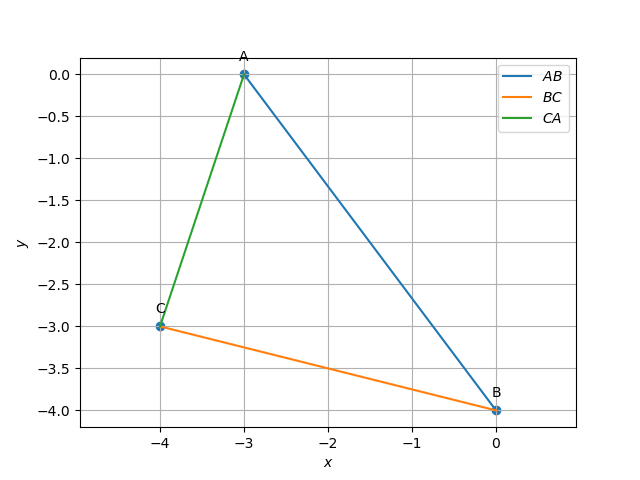
\includegraphics[width=\columnwidth]{./figs/tri.png}
\newpage
\section{MEDIAN}
\begin{tabular}[c]{%
	b{\gnumericColA}%
	b{\gnumericColB}%
	b{\gnumericColC}%
	}
\hhline{|-|-|-}
	 \multicolumn{1}{|p{\gnumericColA}|}%
	{\gnumericPB{\raggedright}\gnumbox[l]{Parameters}}
	&\multicolumn{1}{p{\gnumericColB}|}%
	{\gnumericPB{\raggedright}\gnumbox[l]{Values}}
	&\multicolumn{1}{p{\gnumericColC}|}%
	{\gnumericPB{\centering}\gnumbox[l]{Description}}
\\
\hhline{|---|}
	 \multicolumn{1}{|p{\gnumericColA}|}%
	{\gnumericPB{\raggedright}\gnumbox[l]{$\vec{D}$}}
	&\multicolumn{1}{p{\gnumericColB}|}%
	{\gnumericPB{\raggedright}\gnumbox[l]{$\myvec{-2\\ -\frac{7}{2}}$}}
	&\multicolumn{1}{p{\gnumericColC}|}%
	{\gnumericPB{\centering}\gnumbox[l]{$\frac{\vec{A+B}}{2}$}}
\\
\hhline{|---|}
	 \multicolumn{1}{|p{\gnumericColA}|}%
	{\gnumericPB{\raggedright}\gnumbox[l]{$\vec{E}$}}
	&\multicolumn{1}{p{\gnumericColB}|}%
	{\gnumericPB{\raggedright}\gnumbox[l]{$\myvec{-\frac{7}{2}\\ -\frac{3}{2}}$}}
	&\multicolumn{1}{p{\gnumericColC}|}%
	{\gnumericPB{\centering}\gnumbox[l]{$\frac{\vec{C+A}}{2}$}}
\\
\hhline{|---|}
	 \multicolumn{1}{|p{\gnumericColA}|}%
	{\gnumericPB{\raggedright}\gnumbox[l]{$\vec{F}$}}
	&\multicolumn{1}{p{\gnumericColB}|}%
	{\gnumericPB{\raggedright}\gnumbox[l]{$\myvec{-\frac{3}{2}\\ -2}$}}
	&\multicolumn{1}{p{\gnumericColC}|}%
	{\gnumericPB{\centering}\gnumbox[l]{$\frac{\vec{B+C}}{2}$}}
\\
\hhline{|---|}
	 \multicolumn{1}{|p{\gnumericColA}|}%
	{\gnumericPB{\raggedright}\gnumbox[l]{$\vec{m_4}$}}
	&\multicolumn{1}{p{\gnumericColB}|}%
	{\gnumericPB{\raggedright}\gnumbox[l]{$\myvec{1\\ -\frac{7}{2}}$}}
	&\multicolumn{1}{p{\gnumericColC}|}%
	{\gnumericPB{\centering}\gnumbox[l]{$\vec{D-A}$}}
\\
\hhline{|---|}
	 \multicolumn{1}{|p{\gnumericColA}|}%
	{\gnumericPB{\raggedright}\gnumbox[l]{$\vec{m_5}$}}
	&\multicolumn{1}{p{\gnumericColB}|}%
	{\gnumericPB{\raggedright}\gnumbox[l]{$\myvec{-\frac{7}{2}\\ \frac{5}{2}}$}}
	&\multicolumn{1}{p{\gnumericColC}|}%
	{\gnumericPB{\centering}\gnumbox[l]{$\vec{E-B}$}}
\\
\hhline{|---|}
	 \multicolumn{1}{|p{\gnumericColA}|}%
	{\gnumericPB{\raggedright}\gnumbox[l]{$\vec{m_6}$}}
	&\multicolumn{1}{p{\gnumericColB}|}%
	{\gnumericPB{\raggedright}\gnumbox[l]{$\myvec{\frac{5}{2}\\ 1}$}}
	&\multicolumn{1}{p{\gnumericColC}|}%
	{\gnumericPB{\centering}\gnumbox[l]{$\vec{F-C}$}}
\\
\hhline{|---|}
	 \multicolumn{1}{|p{\gnumericColA}|}%
	{\gnumericPB{\raggedright}\gnumbox[l]{$\vec{n_4}$}}
	&\multicolumn{1}{p{\gnumericColB}|}%
	{\gnumericPB{\raggedright}\gnumbox[l]{$\myvec{-\frac{7}{2}\\ -1}$}}
	&\multicolumn{1}{p{\gnumericColC}|}%
	{\gnumericPB{\centering}\gnumbox[l]{$\myvec{0& 1 \\-1 & 0}\vec{m_4}$}}
\\
\hhline{|---|}
	 \multicolumn{1}{|p{\gnumericColA}|}%
	{\gnumericPB{\raggedright}\gnumbox[l]{$\vec{n_5}$}}
	&\multicolumn{1}{p{\gnumericColB}|}%
	{\gnumericPB{\raggedright}\gnumbox[l]{$\myvec{\frac{5}{2}\\ \frac{7}{2}}$}}
	&\multicolumn{1}{p{\gnumericColC}|}%
	{\gnumericPB{\centering}\gnumbox[l]{$\myvec{0& 1 \\-1 & 0}\vec{m_5}$}}
\\
\hhline{|---|}
	 \multicolumn{1}{|p{\gnumericColA}|}%
	{\gnumericPB{\raggedright}\gnumbox[l]{$\vec{n_6}$}}
	&\multicolumn{1}{p{\gnumericColB}|}%
	{\gnumericPB{\raggedright}\gnumbox[l]{$\myvec{1\\ -\frac{5}{2}}$}}
	&\multicolumn{1}{p{\gnumericColC}|}%
	{\gnumericPB{\centering}\gnumbox[l]{$\myvec{0& 1 \\-1 & 0}\vec{m_6}$}}
\\
\hhline{|---|}
	 \multicolumn{1}{|p{\gnumericColA}|}%
	{\gnumericPB{\raggedright}\gnumbox[l]{$\vec{G}$}}
	&\multicolumn{1}{p{\gnumericColB}|}%
	{\gnumericPB{\raggedright}\gnumbox[l]{$\myvec{-\frac{7}{3}\\ -\frac{7}{3}}$}}
	&\multicolumn{1}{p{\gnumericColC}|}%
	{\gnumericPB{\centering}\gnumbox[l]{$\frac{\vec{A+B+C}}{3}$}}
\\
\hhline{|---|}
	 \multicolumn{1}{|p{\gnumericColA}|}%
	{\gnumericPB{\raggedright}\gnumbox[l]{$\norm{\vec{A-G}}$}}
	&\multicolumn{1}{p{\gnumericColB}|}%
	{\gnumericPB{\raggedright}\gnumbox[l]{$\frac{\sqrt{53}}{3}$}}
	&\multicolumn{1}{p{3\gnumericColC}|}%
	{\setlength{\gnumericMultiRowLength}{0pt}%
	 \addtolength{\gnumericMultiRowLength}{\gnumericColC}%
	 \multirow{6}[3]{\gnumericMultiRowLength}{\parbox{\gnumericMultiRowLength}{%
	 \gnumericPB{\raggedright}\gnumbox[l]{centroid divides median in ratio 2:1}}}}
\\
\hhline{|--|~}
	 \multicolumn{1}{|p{\gnumericColA}|}%
	{\gnumericPB{\raggedright}\gnumbox[l]{$\norm{\vec{D-G}}$}}
	&\multicolumn{1}{p{\gnumericColB}|}%
	{\gnumericPB{\raggedright}\gnumbox[l]{$\frac{\sqrt{53}}{6}$}}
	&\multicolumn{1}{p{\gnumericColC}|}%
	{}
\\
\hhline{|--|~}
	 \multicolumn{1}{|p{\gnumericColA}|}%
	{\gnumericPB{\raggedright}\gnumbox[l]{$\norm{\vec{B-G}}$}}
	&\multicolumn{1}{p{\gnumericColB}|}%
	{\gnumericPB{\raggedright}\gnumbox[l]{$\frac{\sqrt{74}}{3}$}}
	&\multicolumn{1}{p{\gnumericColC}|}%
	{}
\\
\hhline{|--|~}
	 \multicolumn{1}{|p{\gnumericColA}|}%
	{\gnumericPB{\raggedright}\gnumbox[l]{$\norm{\vec{E-G}}$}}
	&\multicolumn{1}{p{\gnumericColB}|}%
	{\gnumericPB{\raggedright}\gnumbox[l]{$\frac{\sqrt{74}}{6}$}}
	&\multicolumn{1}{p{\gnumericColC}|}%
	{}
\\
\hhline{|--|~}
	 \multicolumn{1}{|p{\gnumericColA}|}%
	{\gnumericPB{\raggedright}\gnumbox[l]{$\norm{\vec{C-G}}$}}
	&\multicolumn{1}{p{\gnumericColB}|}%
	{\gnumericPB{\raggedright}\gnumbox[l]{$\frac{\sqrt{29}}{3}$}}
	&\multicolumn{1}{p{\gnumericColC}|}%
	{}
\\
\hhline{|--|~}
	 \multicolumn{1}{|p{\gnumericColA}|}%
	{\gnumericPB{\raggedright}\gnumbox[l]{$\norm{\vec{F-G}}$}}
	&\multicolumn{1}{p{\gnumericColB}|}%
	{\gnumericPB{\raggedright}\gnumbox[l]{$\frac{\sqrt{29}}{6}$}}
	&\multicolumn{1}{p{\gnumericColC}|}%
	{}
\\
\hhline{|---|}
	 \multicolumn{1}{|p{\gnumericColA}|}%
	{\gnumericPB{\raggedright}\gnumbox[l]{rank$\myvec{1& 1& 1 \\ \vec{A}& \vec{D}& \vec{G}}$}}
	&\multicolumn{1}{p{\gnumericColB}|}%
	{\setlength{\gnumericMultiRowLength}{0pt}%
	 \addtolength{\gnumericMultiRowLength}{\gnumericColB}%
	 \multirow{3}[1]{\gnumericMultiRowLength}{\parbox{\gnumericMultiRowLength}{%
	 \gnumericPB{\raggedright}\gnumbox[l]{2}}}}
	&\multicolumn{1}{p{\gnumericColC}|}%
	{\setlength{\gnumericMultiRowLength}{0pt}%
	 \addtolength{\gnumericMultiRowLength}{\gnumericColC}%
	 \multirow{3}[1]{\gnumericMultiRowLength}{\parbox{\gnumericMultiRowLength}{%
	 \gnumericPB{\raggedright}\gnumbox[l]{$\therefore$ points are collinear}}}}
\\
\hhline{|-|~~}
	 \multicolumn{1}{|p{\gnumericColA}|}%
	{\gnumericPB{\raggedright}\gnumbox[l]{rank$\myvec{1& 1& 1 \\ \vec{B}& \vec{E}& \vec{G}}$}}
	&\multicolumn{1}{p{\gnumericColB}|}%
	{}
	&\multicolumn{1}{p{\gnumericColC}|}%
	{}
\\
\hhline{|-|~~}
	 \multicolumn{1}{|p{\gnumericColA}|}%
	{\gnumericPB{\raggedright}\gnumbox[l]{rank$\myvec{1& 1& 1 \\ \vec{C}& \vec{F}& \vec{G}}$}}
	&\multicolumn{1}{p{\gnumericColB}|}%
	{}
	&\multicolumn{1}{p{\gnumericColC}|}%
	{}
\\
\hhline{|---|}
	 \multicolumn{1}{|p{\gnumericColA}|}%
	{\gnumericPB{\raggedright}\gnumbox[l]{AF}}
	&\multicolumn{1}{p{\gnumericColB}|}%
	{\setlength{\gnumericMultiRowLength}{0pt}%
	 \addtolength{\gnumericMultiRowLength}{\gnumericColB}%
	 \multirow{2}[1]{\gnumericMultiRowLength}{\parbox{\gnumericMultiRowLength}{%
	 \gnumericPB{\raggedright}\gnumbox[l]{-3/2, 2}}}}
	&\multicolumn{1}{p{\gnumericColC}|}%
	{\setlength{\gnumericMultiRowLength}{0pt}%
	 \addtolength{\gnumericMultiRowLength}{\gnumericColC}%
	 \multirow{2}[1]{\gnumericMultiRowLength}{\parbox{\gnumericMultiRowLength}{%
	 \gnumericPB{\raggedright}\gnumbox[l]{AFDE is a quad}}}}
\\
\hhline{|-|~~}
	 \multicolumn{1}{|p{\gnumericColA}|}%
	{\gnumericPB{\raggedright}\gnumbox[l]{ED}}
	&\multicolumn{1}{p{\gnumericColB}|}%
	{}
	&\multicolumn{1}{p{\gnumericColC}|}%
	{}
\\
\hhline{|-|-|-|}
\end{tabular}
\clearpage
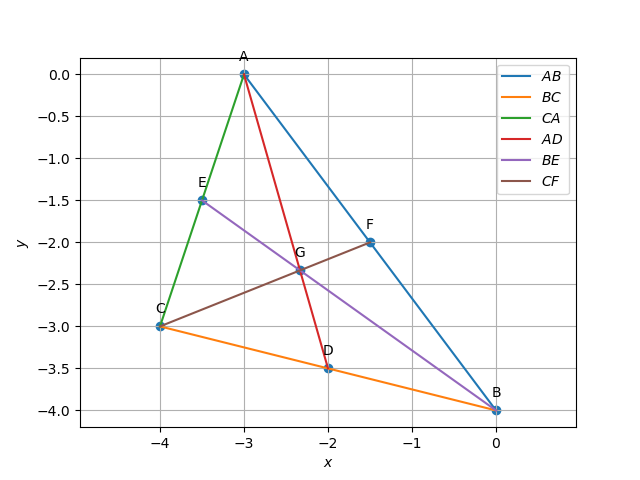
\includegraphics[width=\columnwidth]{./figs/centr.png}
\section{ALTITUDE}
\begin{tabular}[c]{%
	b{\gnumericColA}%
	b{\gnumericColB}%
	b{\gnumericColC}%
	}
\hhline{|-|-|-}
	 \multicolumn{1}{|p{\gnumericColA}|}%
	{\gnumericPB{\raggedright}\gnumbox[l]{Parameters}}
	&\multicolumn{1}{p{\gnumericColB}|}%
	{\gnumericPB{\raggedright}\gnumbox[l]{Values}}
	&\multicolumn{1}{p{\gnumericColC}|}%
	{\gnumericPB{\raggedright}\gnumbox[l]{Description}}
\\
\hhline{|---|}
	 \multicolumn{1}{|p{\gnumericColA}|}%
	{\gnumericPB{\raggedright}\gnumbox[l]{$\vec{n_7}$}}
	&\multicolumn{1}{p{\gnumericColB}|}%
	{\gnumericPB{\raggedright}\gnumbox[l]{$\myvec{-4\\1}$}}
	&\multicolumn{1}{p{\gnumericColC}|}%
	{\gnumericPB{\raggedright}\gnumbox[l]{alt $AD_1$}}
\\
\hhline{|---|}
	 \multicolumn{1}{|p{\gnumericColA}|}%
	{\gnumericPB{\raggedright}\gnumbox[l]{$\vec{n_8}$}}
	&\multicolumn{1}{p{\gnumericColB}|}%
	{\gnumericPB{\raggedright}\gnumbox[l]{$\myvec{1\\3}$}}
	&\multicolumn{1}{p{\gnumericColC}|}%
	{\gnumericPB{\raggedright}\gnumbox[l]{alt $BE_1$}}
\\
\hhline{|---|}
	 \multicolumn{1}{|p{\gnumericColA}|}%
	{\gnumericPB{\raggedright}\gnumbox[l]{$\vec{n_9}$}}
	&\multicolumn{1}{p{\gnumericColB}|}%
	{\gnumericPB{\raggedright}\gnumbox[l]{$\myvec{3\\ -4}$}}
	&\multicolumn{1}{p{\gnumericColC}|}%
	{\gnumericPB{\raggedright}\gnumbox[l]{alt $CF_1$}}
\\
\hhline{|---|}
	 \multicolumn{1}{|p{\gnumericColA}|}%
	{\gnumericPB{\raggedright}\gnumbox[l]{$\vec{H}$}}
	&\multicolumn{1}{p{\gnumericColB}|}%
	{\gnumericPB{\raggedright}\gnumbox[l]{$\myvec{-\frac{48}{13}\\ -\frac{36}{13}}$}}
	&\multicolumn{1}{p{\gnumericColC}|}%
	{\gnumericPB{\raggedright}\gnumbox[l]{orthocentre}}
\\
\hhline{|-|-|-|}
\end{tabular}
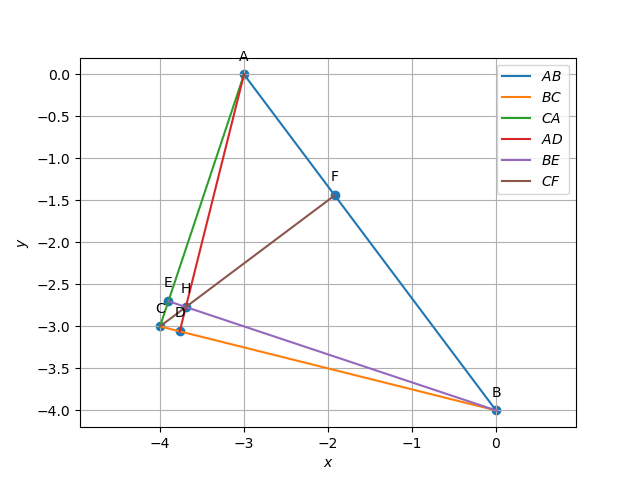
\includegraphics[width=\columnwidth]{./figs/alt.png}
\section{PERPENDICULAR BISECTOR}
\begin{tabular}[c]{%
	b{\gnumericColA}%
	b{\gnumericColB}%
	b{\gnumericColC}%
	}
\hhline{|-|-|-}
	 \multicolumn{1}{|p{\gnumericColA}|}%
	{\gnumericPB{\raggedright}\gnumbox[l]{Parameters}}
	&\multicolumn{1}{p{\gnumericColB}|}%
	{\gnumericPB{\raggedright}\gnumbox[l]{Values}}
	&\multicolumn{1}{p{\gnumericColC}|}%
	{\gnumericPB{\raggedright}\gnumbox[l]{Description}}
\\
\hhline{|---|}
	 \multicolumn{1}{|p{\gnumericColA}|}%
	{\gnumericPB{\raggedright}\gnumbox[l]{$\vec{O}$}}
	&\multicolumn{1}{p{\gnumericColB}|}%
	{\gnumericPB{\raggedright}\gnumbox[l]{$\myvec{-\frac{43}{26}\\ -\frac{55}{26}}$}}
	&\multicolumn{1}{p{\gnumericColC}|}%
	{\gnumericPB{\raggedright}\gnumbox[l]{circumcentre}}
\\
\hhline{|---|}
	 \multicolumn{1}{|p{\gnumericColA}|}%
	{\gnumericPB{\raggedright}\gnumbox[l]{$\norm{\vec{O-A}}$}}
	&\multicolumn{1}{p{\gnumericColB}|}%
	{\setlength{\gnumericMultiRowLength}{0pt}%
	 \addtolength{\gnumericMultiRowLength}{\gnumericColB}%
	 \multirow{3}[1]{\gnumericMultiRowLength}{\parbox{\gnumericMultiRowLength}{%
	 \gnumericPB{\raggedleft}\gnumbox[r]{2.5074}}}}
	&\multicolumn{1}{p{\gnumericColC}|}%
	{\setlength{\gnumericMultiRowLength}{0pt}%
	 \addtolength{\gnumericMultiRowLength}{\gnumericColC}%
	 \multirow{3}[1]{\gnumericMultiRowLength}{\parbox{\gnumericMultiRowLength}{%
	 \gnumericPB{\raggedright}\gnumbox[l]{circumradius}}}}
\\
\hhline{|-|~~}
	 \multicolumn{1}{|p{\gnumericColA}|}%
	{\gnumericPB{\raggedright}\gnumbox[l]{$\norm{\vec{O-B}}$}}
	&\multicolumn{1}{p{\gnumericColB}|}%
	{}
	&\multicolumn{1}{p{\gnumericColC}|}%
	{}
\\
\hhline{|-|~~}
	 \multicolumn{1}{|p{\gnumericColA}|}%
	{\gnumericPB{\raggedright}\gnumbox[l]{$\norm{\vec{O-C}}$}}
	&\multicolumn{1}{p{\gnumericColB}|}%
	{}
	&\multicolumn{1}{p{\gnumericColC}|}%
	{}
\\
\hhline{|-|-|-|}
\end{tabular}	 
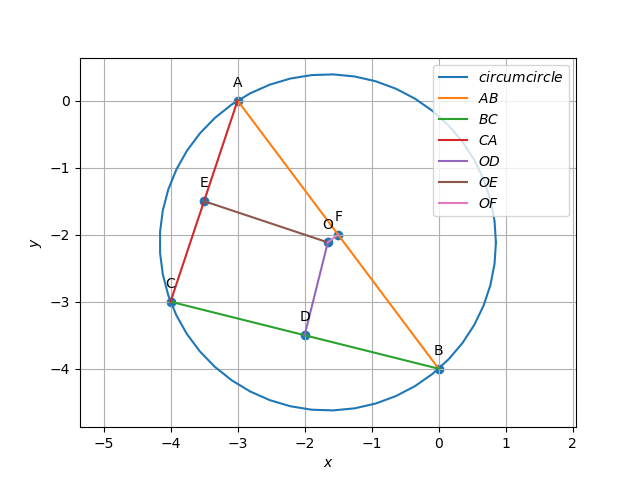
\includegraphics[width=\columnwidth]{./figs/cir.png}
\section{ANGLE BISECTOR}
\begin{tabular}[c]{%
	b{\gnumericColA}%
	b{\gnumericColB}%
	b{\gnumericColC}%
	}
\hhline{|-|-|-}
	 \multicolumn{1}{|p{\gnumericColA}|}%
	{\gnumericPB{\raggedright}\gnumbox[l]{Parameters}}
	&\multicolumn{1}{p{\gnumericColB}|}%
	{\gnumericPB{\raggedright}\gnumbox[l]{Values}}
	&\multicolumn{1}{p{\gnumericColC}|}%
	{\gnumericPB{\raggedright}\gnumbox[l]{Description}}
\\
\hhline{|---|}
	 \multicolumn{1}{|p{\gnumericColA}|}%
	{\gnumericPB{\raggedright}\gnumbox[l]{$\vec{I-A}$}}
	&\multicolumn{1}{p{\gnumericColB}|}%
	{\gnumericPB{\raggedright}\gnumbox[l]{$\myvec{-0.28\\ 1.74}$}}
	&\multicolumn{1}{p{\gnumericColC}|}%
	{\gnumericPB{\raggedright}\gnumbox[l]{angle bisector of $A$}}
\\
\hhline{|---|}
	 \multicolumn{1}{|p{\gnumericColA}|}%
	{\gnumericPB{\raggedright}\gnumbox[l]{$\vec{I-B}$}}
	&\multicolumn{1}{p{\gnumericColB}|}%
	{\gnumericPB{\raggedright}\gnumbox[l]{$\myvec{-1.57\\ 1.04}$}}
	&\multicolumn{1}{p{\gnumericColC}|}%
	{\gnumericPB{\raggedright}\gnumbox[l]{angle bisector of $B$}}
\\
\hhline{|---|}
	 \multicolumn{1}{|p{\gnumericColA}|}%
	{\gnumericPB{\raggedright}\gnumbox[l]{$\vec{I-C}$}}
	&\multicolumn{1}{p{\gnumericColB}|}%
	{\gnumericPB{\raggedright}\gnumbox[l]{$\myvec{-1.28\\ -0.70}$}}
	&\multicolumn{1}{p{\gnumericColC}|}%
	{\gnumericPB{\raggedright}\gnumbox[l]{angle bisector of $C$}}
\\
\hhline{|---|}
	 \multicolumn{1}{|p{\gnumericColA}|}%
	{\gnumericPB{\raggedright}\gnumbox[l]{$\vec{I}$}}
	&\multicolumn{1}{p{\gnumericColB}|}%
	{\gnumericPB{\raggedright}\gnumbox[l]{$\myvec{-2.63\\ -2.25}$}}
	&\multicolumn{1}{p{\gnumericColC}|}%
	{\gnumericPB{\raggedright}\gnumbox[l]{incentre}}
\\
\hhline{|---|}
	 \multicolumn{1}{|p{\gnumericColA}|}%
	{\gnumericPB{\raggedright}\gnumbox[l]{$R_i$}}
	&\multicolumn{1}{p{\gnumericColB}|}%
	{\gnumericPB{\centering}\gnumbox[r]{1.0581}}
	&\multicolumn{1}{p{\gnumericColC}|}%
	{\gnumericPB{\raggedright}\gnumbox[l]{incentre radius}}
\\
\hhline{|---|}
	 \multicolumn{1}{|p{\gnumericColA}|}%
	{\gnumericPB{\raggedright}\gnumbox[l]{$\angle{BAI}$}}
	&\multicolumn{1}{p{\gnumericColB}|}%
	{\setlength{\gnumericMultiRowLength}{0pt}%
	 \addtolength{\gnumericMultiRowLength}{\gnumericColB}%
	 \multirow{2}[1]{\gnumericMultiRowLength}{\parbox{\gnumericMultiRowLength}{%
	 \gnumericPB{\raggedright}\gnumbox[l]{$27.65\degree$}}}}
	&\multicolumn{1}{p{\gnumericColC}|}%
	{\setlength{\gnumericMultiRowLength}{0pt}%
	 \addtolength{\gnumericMultiRowLength}{\gnumericColC}%
	 \multirow{2}[1]{\gnumericMultiRowLength}{\parbox{\gnumericMultiRowLength}{%
	 \gnumericPB{\raggedright}\gnumbox[l]{bisector of $A$}}}}
\\
\hhline{|-|~~}
	 \multicolumn{1}{|p{\gnumericColA}|}%
	{\gnumericPB{\raggedright}\gnumbox[l]{$\angle{CAI}$}}
	&\multicolumn{1}{p{\gnumericColB}|}%
	{}
	&\multicolumn{1}{p{\gnumericColC}|}%
	{}
\\
\hhline{|---|}
	 \multicolumn{1}{|p{\gnumericColA}|}%
	{\gnumericPB{\raggedright}\gnumbox[l]{$\angle{ABI}$}}
	&\multicolumn{1}{p{\gnumericColB}|}%
	{\setlength{\gnumericMultiRowLength}{0pt}%
	 \addtolength{\gnumericMultiRowLength}{\gnumericColB}%
	 \multirow{2}[1]{\gnumericMultiRowLength}{\parbox{\gnumericMultiRowLength}{%
	 \gnumericPB{\raggedright}\gnumbox[l]{$19.54\degree$}}}}
	&\multicolumn{1}{p{\gnumericColC}|}%
	{\setlength{\gnumericMultiRowLength}{0pt}%
	 \addtolength{\gnumericMultiRowLength}{\gnumericColC}%
	 \multirow{2}[1]{\gnumericMultiRowLength}{\parbox{\gnumericMultiRowLength}{%
	 \gnumericPB{\raggedright}\gnumbox[l]{bisector of $B$}}}}
\\
\hhline{|-|~~}
	 \multicolumn{1}{|p{\gnumericColA}|}%
	{\gnumericPB{\raggedright}\gnumbox[l]{$\angle{CBI}$}}
	&\multicolumn{1}{p{\gnumericColB}|}%
	{}
	&\multicolumn{1}{p{\gnumericColC}|}%
	{}
\\
\hhline{|---|}
	 \multicolumn{1}{|p{\gnumericColA}|}%
	{\gnumericPB{\raggedright}\gnumbox[l]{$\angle{BCI}$}}
	&\multicolumn{1}{p{\gnumericColB}|}%
	{\setlength{\gnumericMultiRowLength}{0pt}%
	 \addtolength{\gnumericMultiRowLength}{\gnumericColB}%
	 \multirow{2}[1]{\gnumericMultiRowLength}{\parbox{\gnumericMultiRowLength}{%
	 \gnumericPB{\raggedright}\gnumbox[l]{$137.12\degree$}}}}
	&\multicolumn{1}{p{\gnumericColC}|}%
	{\setlength{\gnumericMultiRowLength}{0pt}%
	 \addtolength{\gnumericMultiRowLength}{\gnumericColC}%
	 \multirow{2}[1]{\gnumericMultiRowLength}{\parbox{\gnumericMultiRowLength}{%
	 \gnumericPB{\raggedright}\gnumbox[l]{bisector of $C$}}}}
\\
\hhline{|-|~~}
	 \multicolumn{1}{|p{\gnumericColA}|}%
	{\gnumericPB{\raggedright}\gnumbox[l]{$\angle{ACI}$}}
	&\multicolumn{1}{p{\gnumericColB}|}%
	{}
	&\multicolumn{1}{p{\gnumericColC}|}%
	{}
\\
\hhline{|---|}
	 \multicolumn{1}{|p{\gnumericColA}|}%
	{\gnumericPB{\raggedright}\gnumbox[l]{$\vec{D_3}$}}
	&\multicolumn{1}{p{\gnumericColB}|}%
	{\gnumericPB{\raggedright}\gnumbox[l]{$\myvec{-2.89\\ -3.27}$}}
	&\multicolumn{1}{p{1.7\gnumericColC}|}%
	{\setlength{\gnumericMultiRowLength}{0pt}%
	 \addtolength{\gnumericMultiRowLength}{\gnumericColC}%
	 \multirow{3}[1]{\gnumericMultiRowLength}{\parbox{\gnumericMultiRowLength}{%
	 \gnumericPB{\raggedright}\gnumbox[l]{points of intersection}}}}
\\
\hhline{|--|~}
	 \multicolumn{1}{|p{\gnumericColA}|}%
	{\gnumericPB{\raggedright}\gnumbox[l]{$\vec{E_3}$}}
	&\multicolumn{1}{p{\gnumericColB}|}%
	{\gnumericPB{\raggedright}\gnumbox[l]{$\myvec{-1.78\\ -1.61}$}}
	&\multicolumn{1}{p{\gnumericColC}|}%
	{}
\\
\hhline{|--|~}
	 \multicolumn{1}{|p{\gnumericColA}|}%
	{\gnumericPB{\raggedright}\gnumbox[l]{$\vec{F_3}$}}
	&\multicolumn{1}{p{\gnumericColB}|}%
	{\gnumericPB{\raggedright}\gnumbox[l]{$\myvec{-2.89\\ -3.27}$}}
	&\multicolumn{1}{p{\gnumericColC}|}%
	{}
\\
\hhline{|-|-|-|}
\end{tabular}
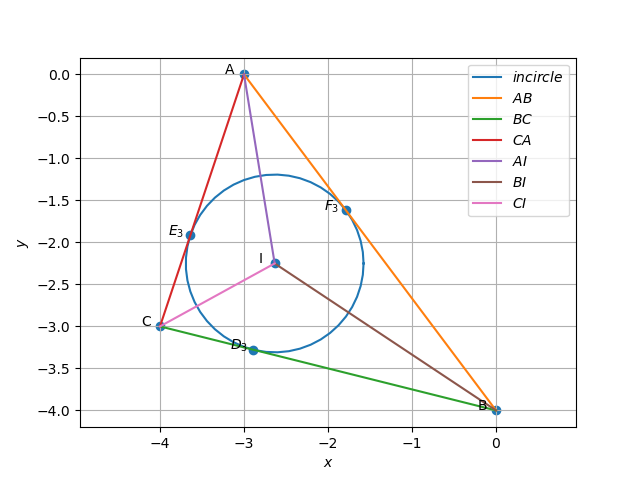
\includegraphics[width=\columnwidth]{./figs/incir.png}
\ifthenelse{\isundefined{\languageshorthands}}{}{\languageshorthands{\languagename}}
\gnumericTableEnd
